\setcounter{chapter}{1}
\chapter{O que é User Experience (UX)}

\begin{flushright}
	\textit{
		UX é pesquisar sobre os usuários de modo que você possa dar para eles \\ o que eles precisam para conseguirem algo que querem.
	} \\
	
	\textbf{autor desconhecido}
\end{flushright}


No Capítulo \ref{cap:cap1}, nós realizamos a introdução sobre alguns conceitos norteadores da Interação Humano-Computador (IHC). No meio de todos os conceitos apresentados, algo se destaca em meio ao material apresentado, que é \textbf{usuário}. Sem dúvida, podemos afirmar que, o usuário, mediante sua interação com os sistemas computacionais, é a base para que uma área de estudo como IHC pudesse ser construída.

Já neste capítulo, iremos tratar não somente da interação do usuário por meios das interfaces, mas também da qualidade da sua experiência ao usar elas.

\section{Experiência do usuário}

Segundo \citeonline{teixeira2014introduccao}, a experiência do usuário existe desde que o mundo é mundo. Desde que as pessoas começaram a ``usar' objetos para realizar alguma tarefa podemos dizer que existe um contexto de experiências. Experiências são subjetivas. Cada pessoa tem uma experiência diferente ao usar um caixa eletrônico, um aplicativo, uma rede social, entre outros. Essa experiência, segundo \citeonline{teixeira2014introduccao} é influenciada por dois tipos de fatores: \textbf{humanos} e \textbf{externos} 

Como \textbf{fatores humanos} podemos citar as habilidade em usar caixas eletrônicos, por exemplo. Sua visão, sua habilidade motora, sua capacidade de ler e entender o que está escrito na tela, seu humor naquele momento, entre outros fatos. Já como \textbf{fatores externos}, podemos citar o horário do dia, o ambiente onde o caixa eletrônico está instalado, o fato de ter uma fila de pessoas atrás do utilizador, e assim por diante.

Assim, podemos dizer que o tema experiência do usuário é um tema bastante subjetivo. É difícil de maneira objetiva e direta dizer como desenhar uma experiência do usuário, mas é possível aprendermos como desenhar um produto, serviço ou ambiente que proporcione uma experiência satisfatória para alguém que os use, identificando todos os aspectos da interação do usuário com esse produto (ou serviço ou ambiente).

Portanto, a experiência do usuário está ligado a forma com que a pessoa se sente ao usar um produto. Ou mais formalmente, de acordo com a definição dada pela ISO 9241-210, são as respostas e percepções de uma pessoa resultantes do uso de um produto, sistema ou serviço.

UX designers trabalham para construir produtos que sejam fáceis de usar
(a tal \textbf{usabilidade}), reduzindo a fricção e permitindo que os usuários completem a tarefa desejada em menos tempo, com menos ruído e obstáculos.

\begin{figure}[H]
	\centering
	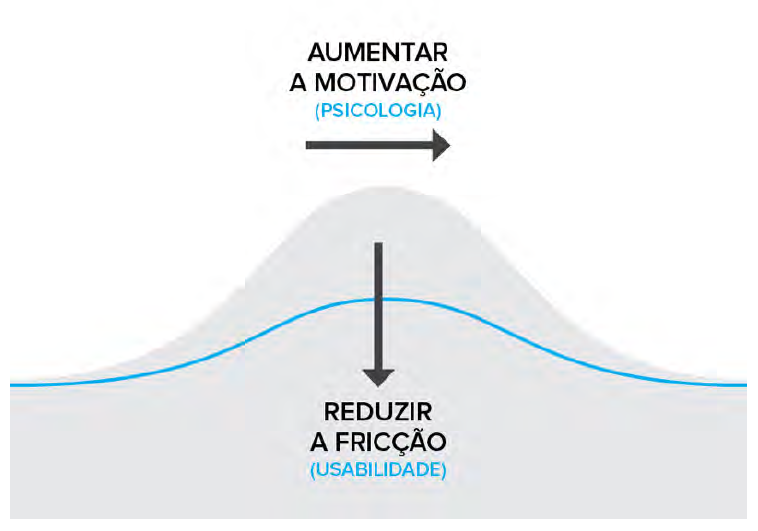
\includegraphics[scale=0.4]{imagens/aumento-friqcao.png}
	\caption{Stephen Anderson. Livro Seductive Interaction Design}
	%\legend{Fonte: \cite{IrlaRebelo}}
	%\label{fig:interface-interacao}
\end{figure}

\subsection{Usabilidade e a experiência do usuário}

Segundo a norma sobre requisitos de ergonomia, ISO 9241-11 (1998), define usabilidade como sendo: \textit{O grau em que um produto é usado por usuários específicos para atingir objetivos
específicos com \textbf{eficácia}, \textbf{eficiência} e \textbf{satisfação} em um contexto de uso
específico.}

\begin{itemize}
	\item \textbf{eficácia}: está relacionada com a capacidade de os usuários interagirem com o sistema para alcançar seus objetivos corretamente, conforme o esperado;
	
	\item \textbf{eficiência}:  está relacionada com os recursos necessários para os usuários
	interagirem com o sistema e alcançarem seus objetivos. Normalmente, os recursos
	necessários são tempo, mão de obra e materiais envolvidos; 
	
	\item \textbf{satisfação}: A norma também destaca
	a importância de considerarmos o grau de contentamento dos usuários com a experiência
	de usar o sistema interativo no contexto de uso para o qual foi projetado.
\end{itemize} 

De forma mais simplificada, segundo \cite{teixeira2014introduccao}: usablidade é garantir que as interfaces sejam fáceis de usar. Que o usuário consiga realizar uma tarefa sem transtorno ou demora em um número
razoável de passos, como também, toda informações sejam fáceis de entender e de fácil acesso. 

\section{Métodos e entregáveis em UX}

Quando falamos em métodos e entregáveis, os profissionais da área costumam ter uma série itens que gostam de utilizar: wireframes, sitemaps, user journeys, análise comparativa de funcionalidades, entre vários outros. Contudo, neste capítulo, vamos abordar apenas três os quais acreditamos ser os mais utilizados que são: \textbf{Brainstorming, Personas, Entrevistas com Stakeholders, Wireframes e Sitemaps}.

\subsection{Brainstorming}

O processo coletivo de geração de ideias, sem restrições. Uma sessão de \textit{brainstorming} busca
levantar de forma bastante livre um conjunto grande e abrangente de opiniões dos
participantes em torno de um tema. Os resultados dessa atividade podem alimentar
diretamente a especificação funcional e documentação de design \cite{barbosa2010IHC}.

\subsection{Personas}

Para \citeonline{teixeira2014introduccao}, personas é  um retrato do público-alvo que destaca dados demográficos, comportamentos,
necessidades e motivações por meio da criação de um personagem ficcional
baseado em \textit{insights} extraídos de pesquisa. Personas fazem com que os designers e desenvolvedores criem empatia com os consumidores durante o processo de design.

\begin{figure}[H]
	\centering
	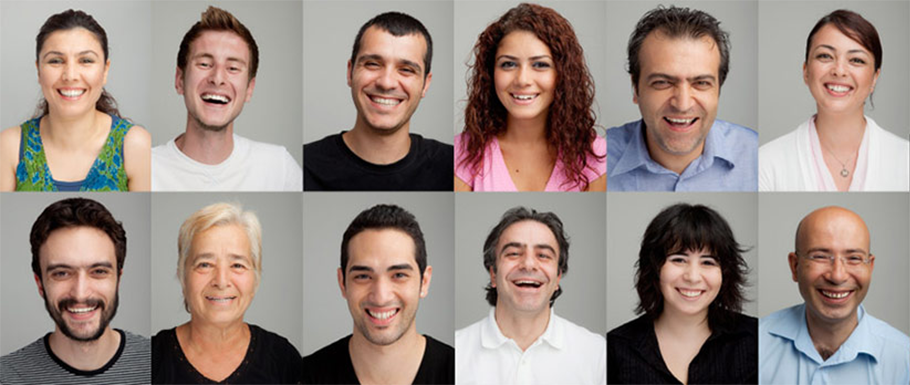
\includegraphics[scale=0.4]{imagens/personas-marketing.png}
	\caption{Exemplo de personas}
	\legend{Fonte: http://www.altgrupo.com.br/blog/marketing-digital-por-que-investir-no-uso-de-personas/}
	%\label{fig:interface-interacao}
\end{figure}

Para definir uma persona, \citeonline{courage2005understanding} enumera os seguintes elementos característicos:

\begin{itemize}
	\item \textbf{identidade}: dê a uma persona nome e sobrenome. Forneça uma idade e outros dados demográficos que seriam representativos do perfil do usuário. Inclua também uma foto, para tornar a persona ainda mais realista e memorável;
	\item \textbf{status}: defina se esta persona é primária, secundária, outro \textit{stakeholder} ou representa um antiusuário do seu sistema. Um antiusuário é alguém que não vai utilizar o produto e, portanto, não deve influenciar as decisões de projeto;
	\item \textbf{objetivos}: quais são os objetivos desta persona? Não se limite a objetivos relacionados ao seu produto específico;
	\item \textbf{habilidades}: qual é a especialidade da sua persona? Isso inclui educação, treinamento e competências específicas. Novamente, não se limite a detalhes relacionados ao seu produto específico;
	\item \textbf{tarefas}: em linhas gerais, quais as tarefas básicas ou críticas que a persona realiza? Qual é a frequência, importância e duração dessas tarefas?;
	\item \textbf{relacionamentos}: entender com quem a persona se relaciona é importante, pois ajuda a identificar outros \textit{stakeholders};
	\item \textbf{requisitos}: de que a persona precisa? Inclua citações que ajudam a dar mais vida a essas necessidades;
	\item \textbf{expectativas}: como a persona acredita que o produto funciona? Como ela organiza as informações no seu domínio ou trabalho?
\end{itemize}

Embora personas sejam fictícias, elas são definidas com rigor e detalhes para representar usuários ``típicos''. Elas são derivadas de um processo de investigação que levanta as características dos usuários e descreve seus perfis \cite{barbosa2010IHC}.

\subsubsection{Diferença entre persona e público-alvo}

Para \citeonline{riandutra2018} um erro bastante esta no fato da não diferenciação de personas de público-alvo. O público-alvo é algo mais genérico, abrangente, enquanto a persona é mais humanizada e personalizada.

Por exemplo, um público-alvo poderia ser: homens e mulheres, entre 30 e 40 anos, casados, com ensino médio completo, com renda mensal de até 15.000 reais. Têm até dois filhos e pretendem comprar uma casa de veraneio para a família.

Agora, um exemplo de persona: Patrícia, 31 anos, não tem filhos, é solteira, formada em design e pós-graduada em animação 3D. Busca ascensão profissional na empresa em que trabalha há cerca de dois anos. Gostaria de morar sozinha e procura formas de poupar dinheiro para as despesas de um novo apartamento.




